\chapter{Evaluation}
This chapter is the evaluation of the script based on the Google Lighthouse audit. This chapter will highlight some elements of the audit. The full audit can be seen in appendix x. The given score in the relevant categories can be seen in figure x. There was a bug in the measurement of the performance score, which will be further expanded upon in section x. This means that the tool. It does however still provide some useful suggestions as to how the site could be improved.




\begin{figure} [H]
	\centering
	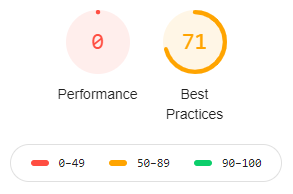
\includegraphics[width=.8\textwidth]{Pictures/LighthouseGrade}
	\caption{The score for performance and best pratices from Google Lighthouse}
	\label{LighthouseGrade}
\end{figure}

\subsection{Performance}
As shown the performance scored nothing out of a hundred. The performance in each of the metrics can be seen in figure x.

\begin{figure} [H]
	\centering
	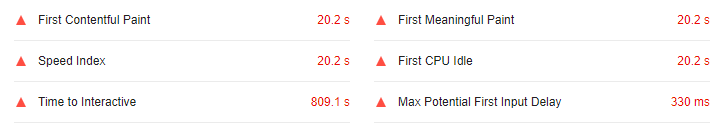
\includegraphics[width=.8\textwidth]{Pictures/PerformanceAuditValues}
	\caption{The result of the performance audit}
	\label{PerformanceAuditValues}
\end{figure}

\fxnote{Write that it is nonsense}

\subsection{Opportunities}
In addition to providing the metrics for the performance Lighthouse also comes with suggestion to how the loading time can be reduced. 
\textbf{Eliminate render-blocking resources}
The opportunity for the largest estimated time saving is to eliminate render-blocking resources. These are the URLs, which must be loaded before the first paint can be applied to the page. 
https://web.dev/render-blocking-resources/?utm_source=lighthouse&utm_medium=devtools

Table x shows the different libraries, which have to be loaded before the site is rendered. It can be seen that Openlayers is 82 \% of the loaded data.
\fxnote{Have I written about Jquery??}

\begin{table}[htbp]
	\centering
	\begin{tabular}{l}
		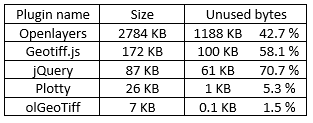
\includegraphics[width=0.8\textwidth]{Pictures/tabPluginSize}
	\end{tabular}
	\caption{Size of loaded modules and the much they are used}
	\label{tabPluginSize}
\end{table}

When analysed further with the Coverage tool it can be seen that a large part of the Openlayers library is not being used as show in table \ref{tabPluginSize}.  
\fxnote{TODO: Make a table from the information in the figure below – tabtext – resourse use of the 3 larges libraries}

\fxnote{Write about Coverage earlier – maybe in evaluation tools}

\textbf{Minification and compressing}
Files sizes and script parsing time can be reduced by minifying and compressing the files. 

A minified file is a file, where all the unnecessary parts have been cut away. Whitespaces and unused code are removed leaving a smaller file, which still functions perfectly. 

Compression is using an algorithm to modify the data, so that it takes up less space.
https://web.dev/unminified-javascript/?utm_source=lighthouse&utm_medium=devtools
\fxnote{For exam: Try using Terser to minify and compress – Write about Terser in future work}
\textbf{Avoid enormous network payloads}
Long loading times are highly correlated with the amount of loaded data.  
https://web.dev/total-byte-weight/?utm_source=lighthouse&utm_medium=devtools
Loading the raster tiles for the map does require loading multiple files with a large bit depth, which requires a lengthy loading time. 

\textbf{Does not use HTTP/2 for all of its resources}
This suggested improvement appears if some of the page’s resources are being served with a version of HTTP/1. According to Google Audit all loaded resources are being delivered using HTTP 1.1.

\fxnote{Write about HTTP/2 earlier?}

https://web.dev/uses-http2/?utm_source=lighthouse&utm_medium=devtools

\textbf{Uses deprecated APIs}
When loading the metadata about the tiles a synchronous XMLRequest is used. This is a deprecated API, which will be removed from Chrome in a feature edition. 
https://web.dev/deprecations/?utm_source=lighthouse&utm_medium=devtools
